\section{Field Cage} \label{sec:Introduction} 


The NEXT-DEMO field cage is designed to provide an homogeneous and uniform electric field inside the active volume of the NEXT-DEMO detector. To achieve this different parts have to be designed, constructed and assembled. The different components of the the field cage project are:
\begin{itemize}
\item Drift region.
\item Buffer.
\item High voltage feedthroughs.
\item Cathode grid.
\item Electroluminescent region.
\end{itemize}


The main safety issues are related with the high voltage that we need to apply to the detector. In that sense, the entire detector and all of its metallic components are to be grounded for safety. The grounding points will provide path of least resistance to any stray transients resulting from HV discharges as is common for operation of HV equipment. Moreover, the currents will be small ($\mathcal{O}(\mu A)$) due to the large value of the resistors involved.

\subsection{Drift region}

The drift regions needs to create a moderate (300-600V/cm) but very homogeneous electric field. This is done using copper rings connected 10$G\Omega$ resistors. Figure \ref{fig:drift1} shows an example of the rings used for the NEW detector, the concept used in DEMO will be the same.

\begin{figure}[h!]
\centering
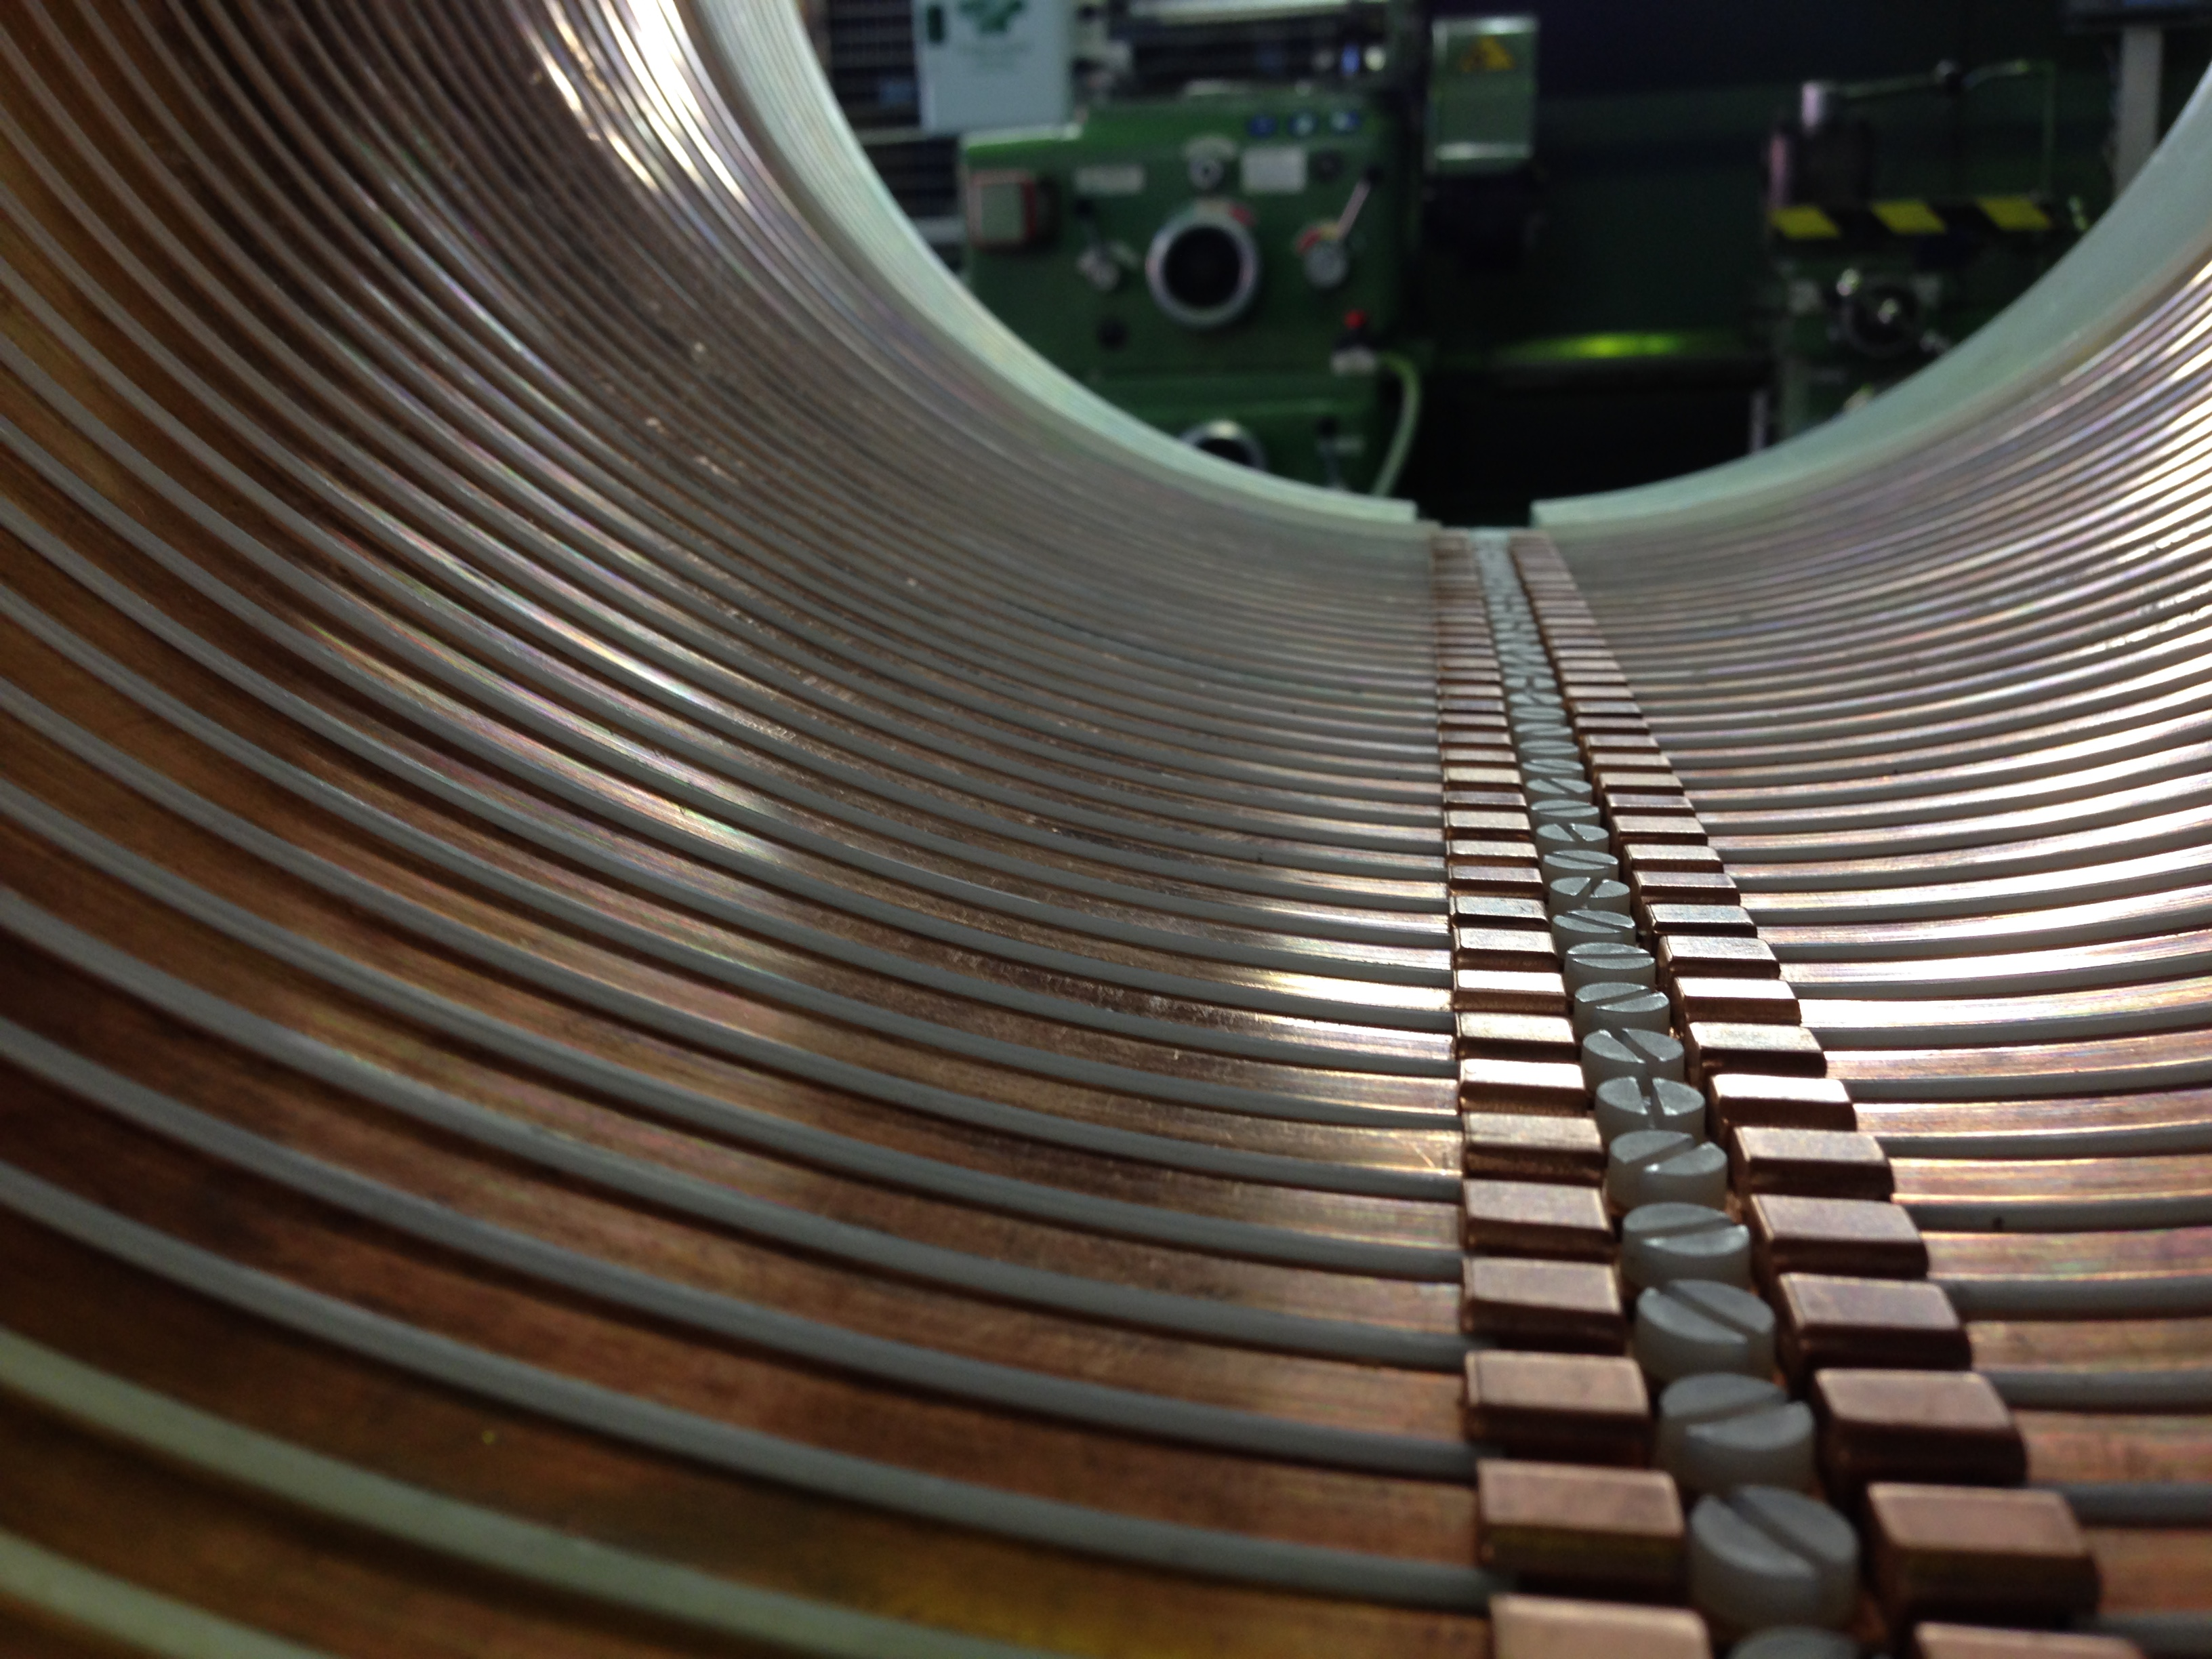
\includegraphics[height=8cm]{img/IMG_0246.JPG}
\caption{Detail of the copper rings in the drift region.} \label{fig:drift1}
\end{figure}


\subsection{Buffer region}

In order to protect the PMTs' windows from the cathode voltage safely a certain distance is needed. This space is what we call buffer region. In the current design the buffer region consists in a structure made completely with High Density Polyethilene (HDPE). The electric field in this region is much higher than in the drift region, as much as 5kV/cm, and it can result in sparks in different parts of the detector. For that reason the buffer has been extensively tested and has demostrated to be very robust and stable.

%A first test using a small set-up has shown promising result. The buffer region held the voltage until the High Voltage Feedthrough used for the test started sparking (Fig. \ref{fig:buff1}).
%
%\begin{figure}[h!]
%\centering
%\includegraphics[width=0.45\textwidth]{img/buff1.JPG}
%\caption{Detail of the buffer region test made with High Density Polyethilene (HDPE). Carbon tracks appear to the outside of the HDPE but no carbon tracks are visible in the inside of the buffer region. } \label{fig:buff1}
%\end{figure}
%
%A more extensive and realistic test will be performed using the NEXT-DEMO detector. For conducting this test we will replace the current NEXT-DEMO field cage by a small scale field cage of NEW (Fig. \ref{fig:bufftest}) using also the same HVFT that we want to use for NEW. In this way we would be able to test time both the buffer region and the HVFT in a more realistic situation.
%
%\begin{figure}[h!]
%\centering
%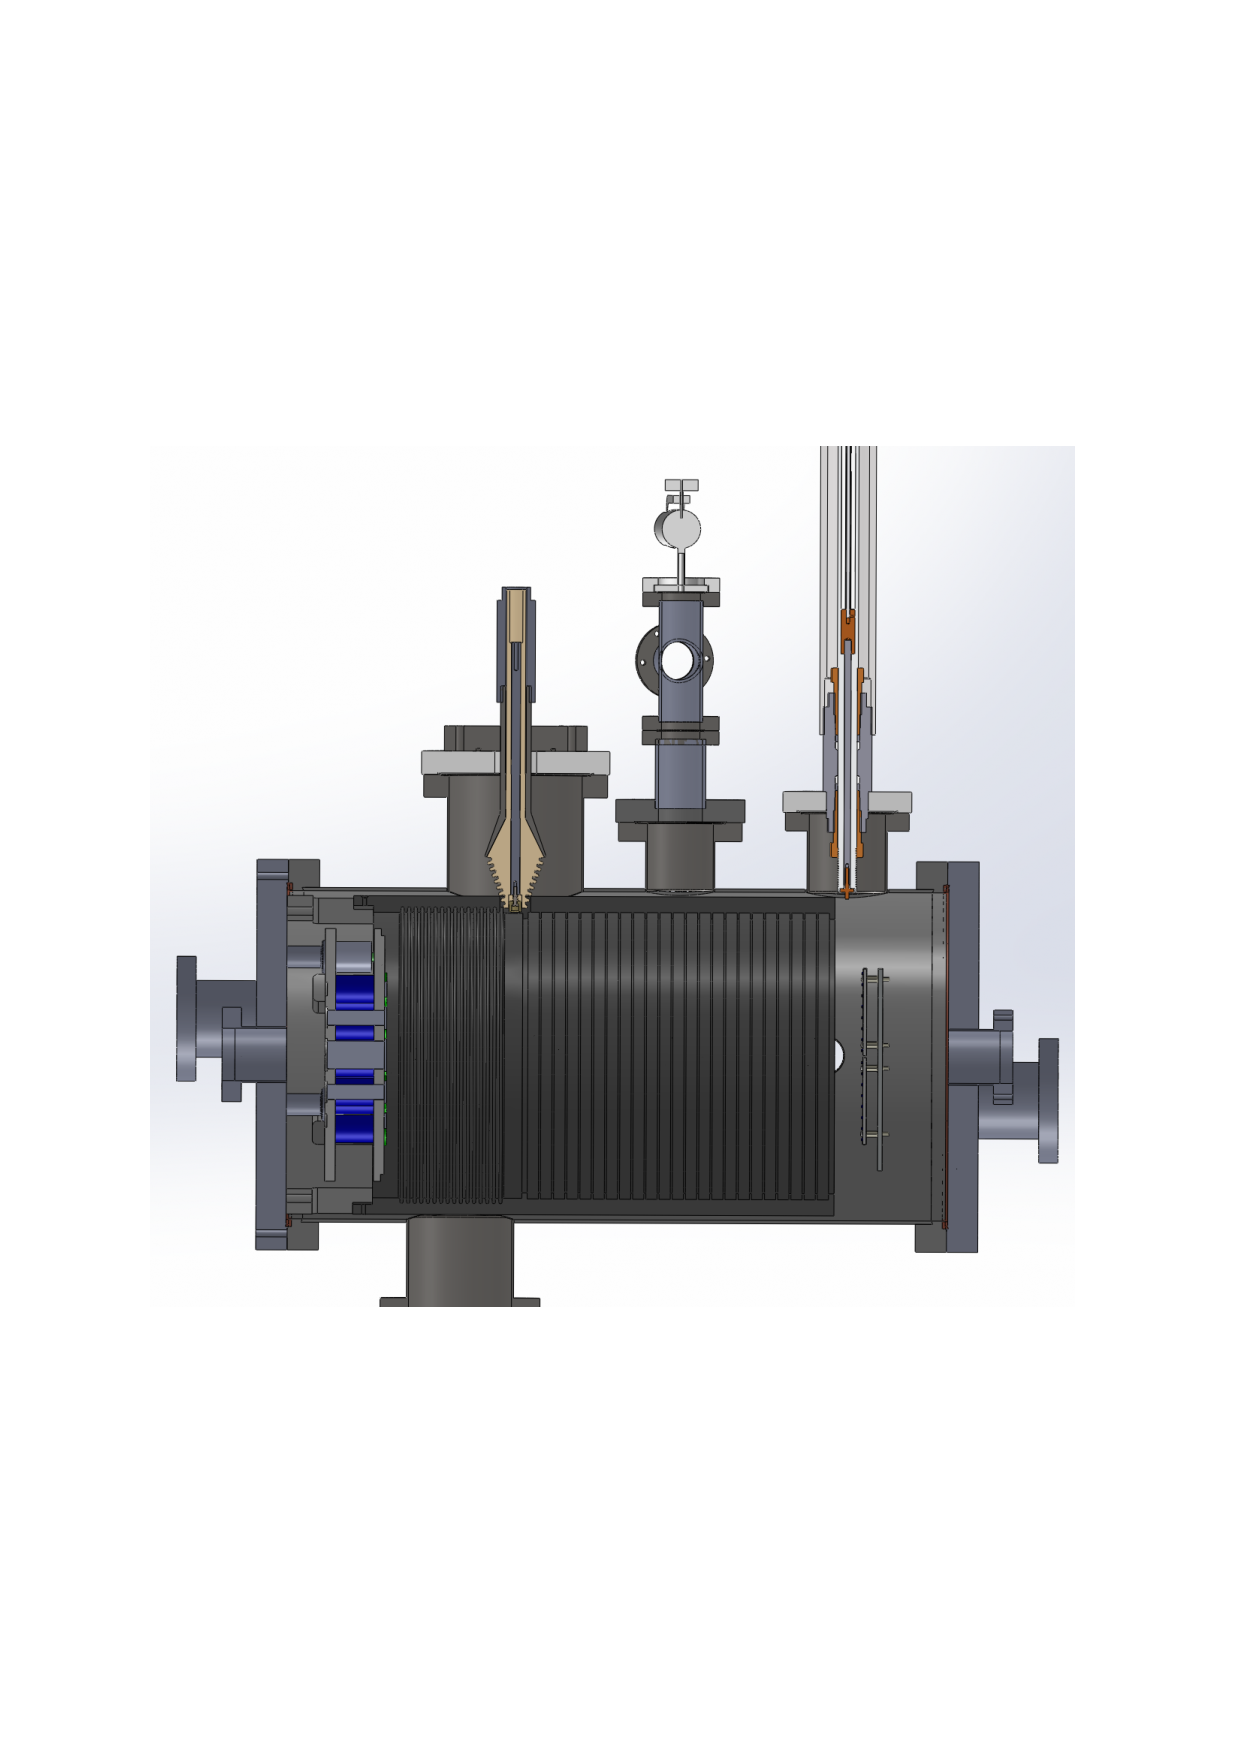
\includegraphics[width=0.45\textwidth]{img/demotest}
%\caption{Design of the test to be performed in the NEXT-DEMO detector. In the cathode (left) the feedthrough with the NEW design is used, in the gate (right) the feedthrough currently being used in DEMO is shown as reference.} \label{fig:bufftest}
%\end{figure}


\subsection{High voltage feedthroughs}

In order to create the different field regions high voltage has to be applied in different parts of the detector. Due to the impossibility of generating the high voltage (HHV) inside the detector (due radioactivity and space problems), the HHV has to be produced outside and then passed inside using feedthroughs that passes the voltage but stops gas leaks.

When discussing about feedthroughs we should differentiate three parts: The high voltage modules, the cable and the feedthrough itself.

Figure \ref{fig:hvft1}) shows the design and the results of the electric field simulations.

\begin{figure}[h!]
\centering
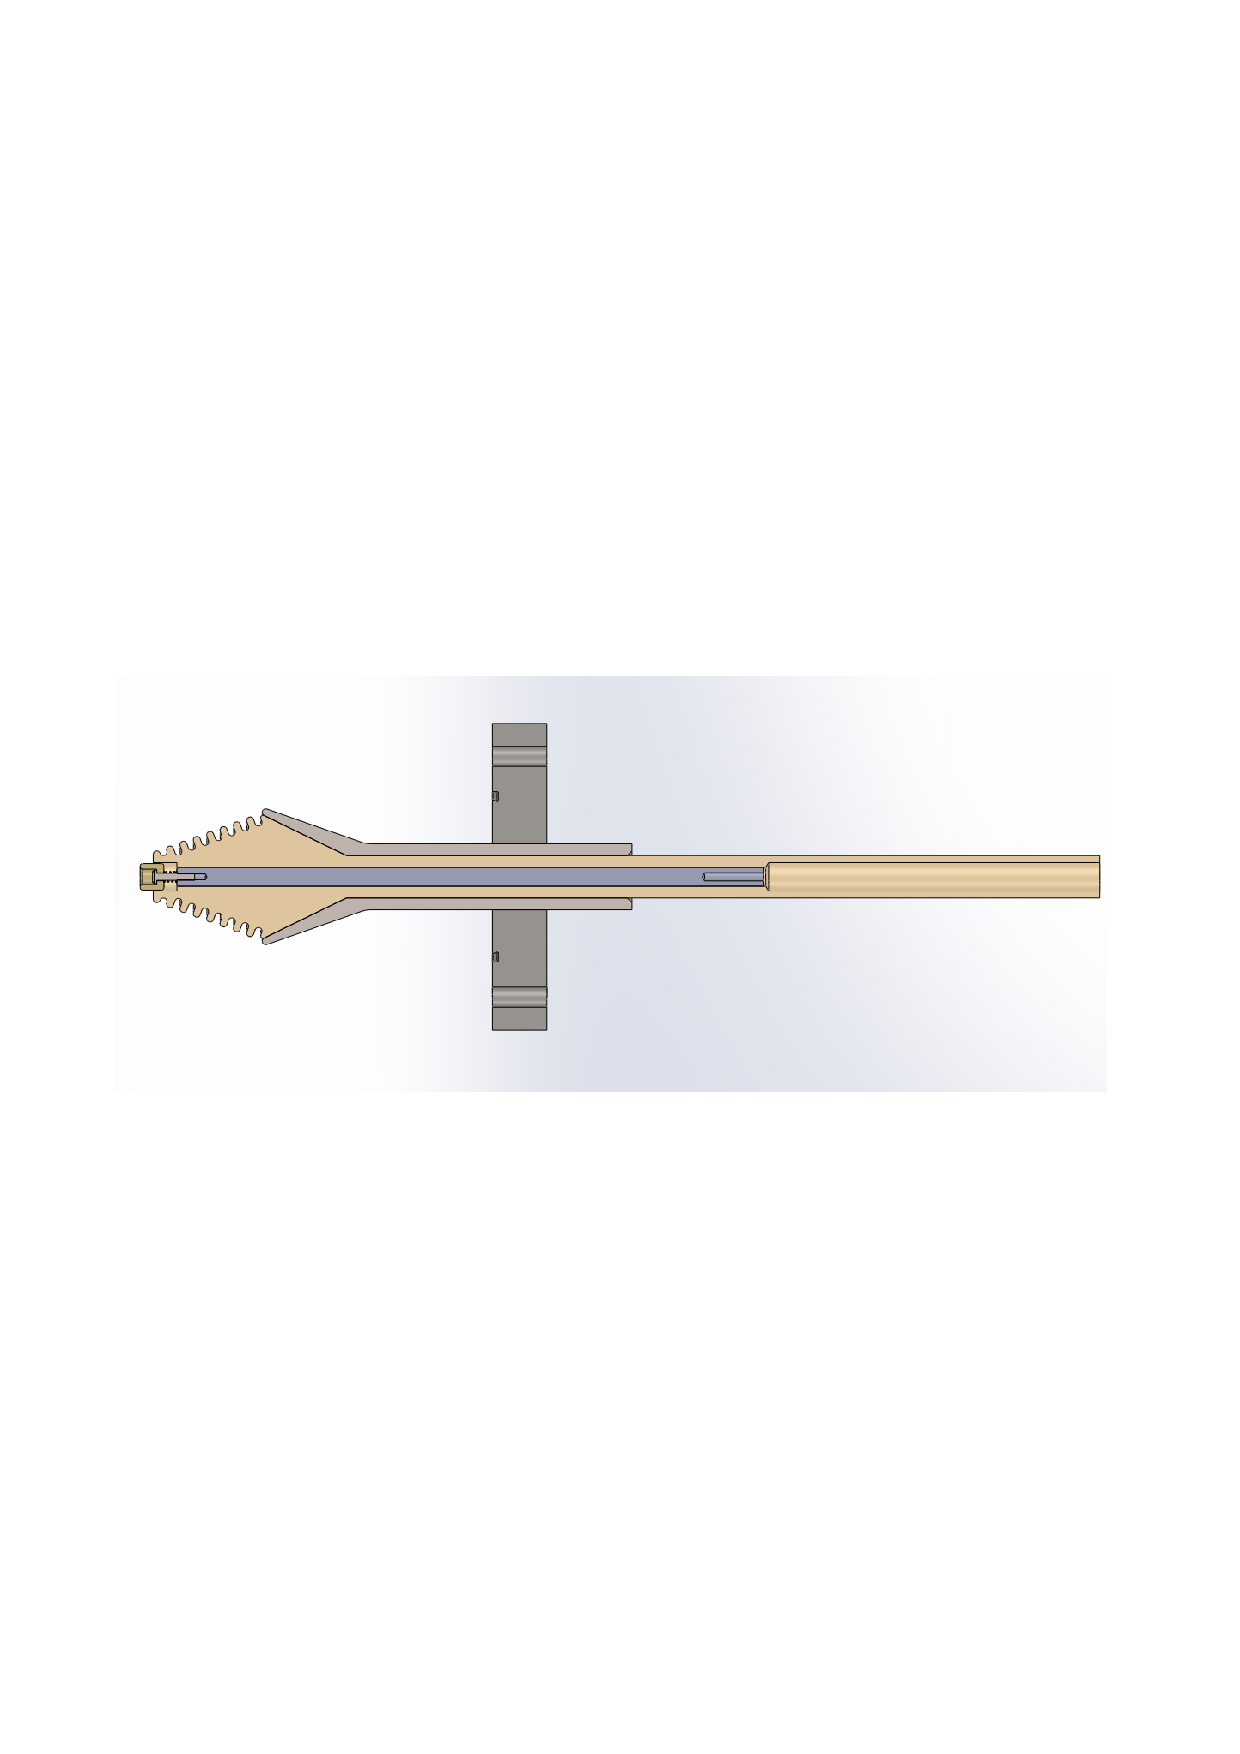
\includegraphics[width=0.45\textwidth]{img/hvft1.pdf}
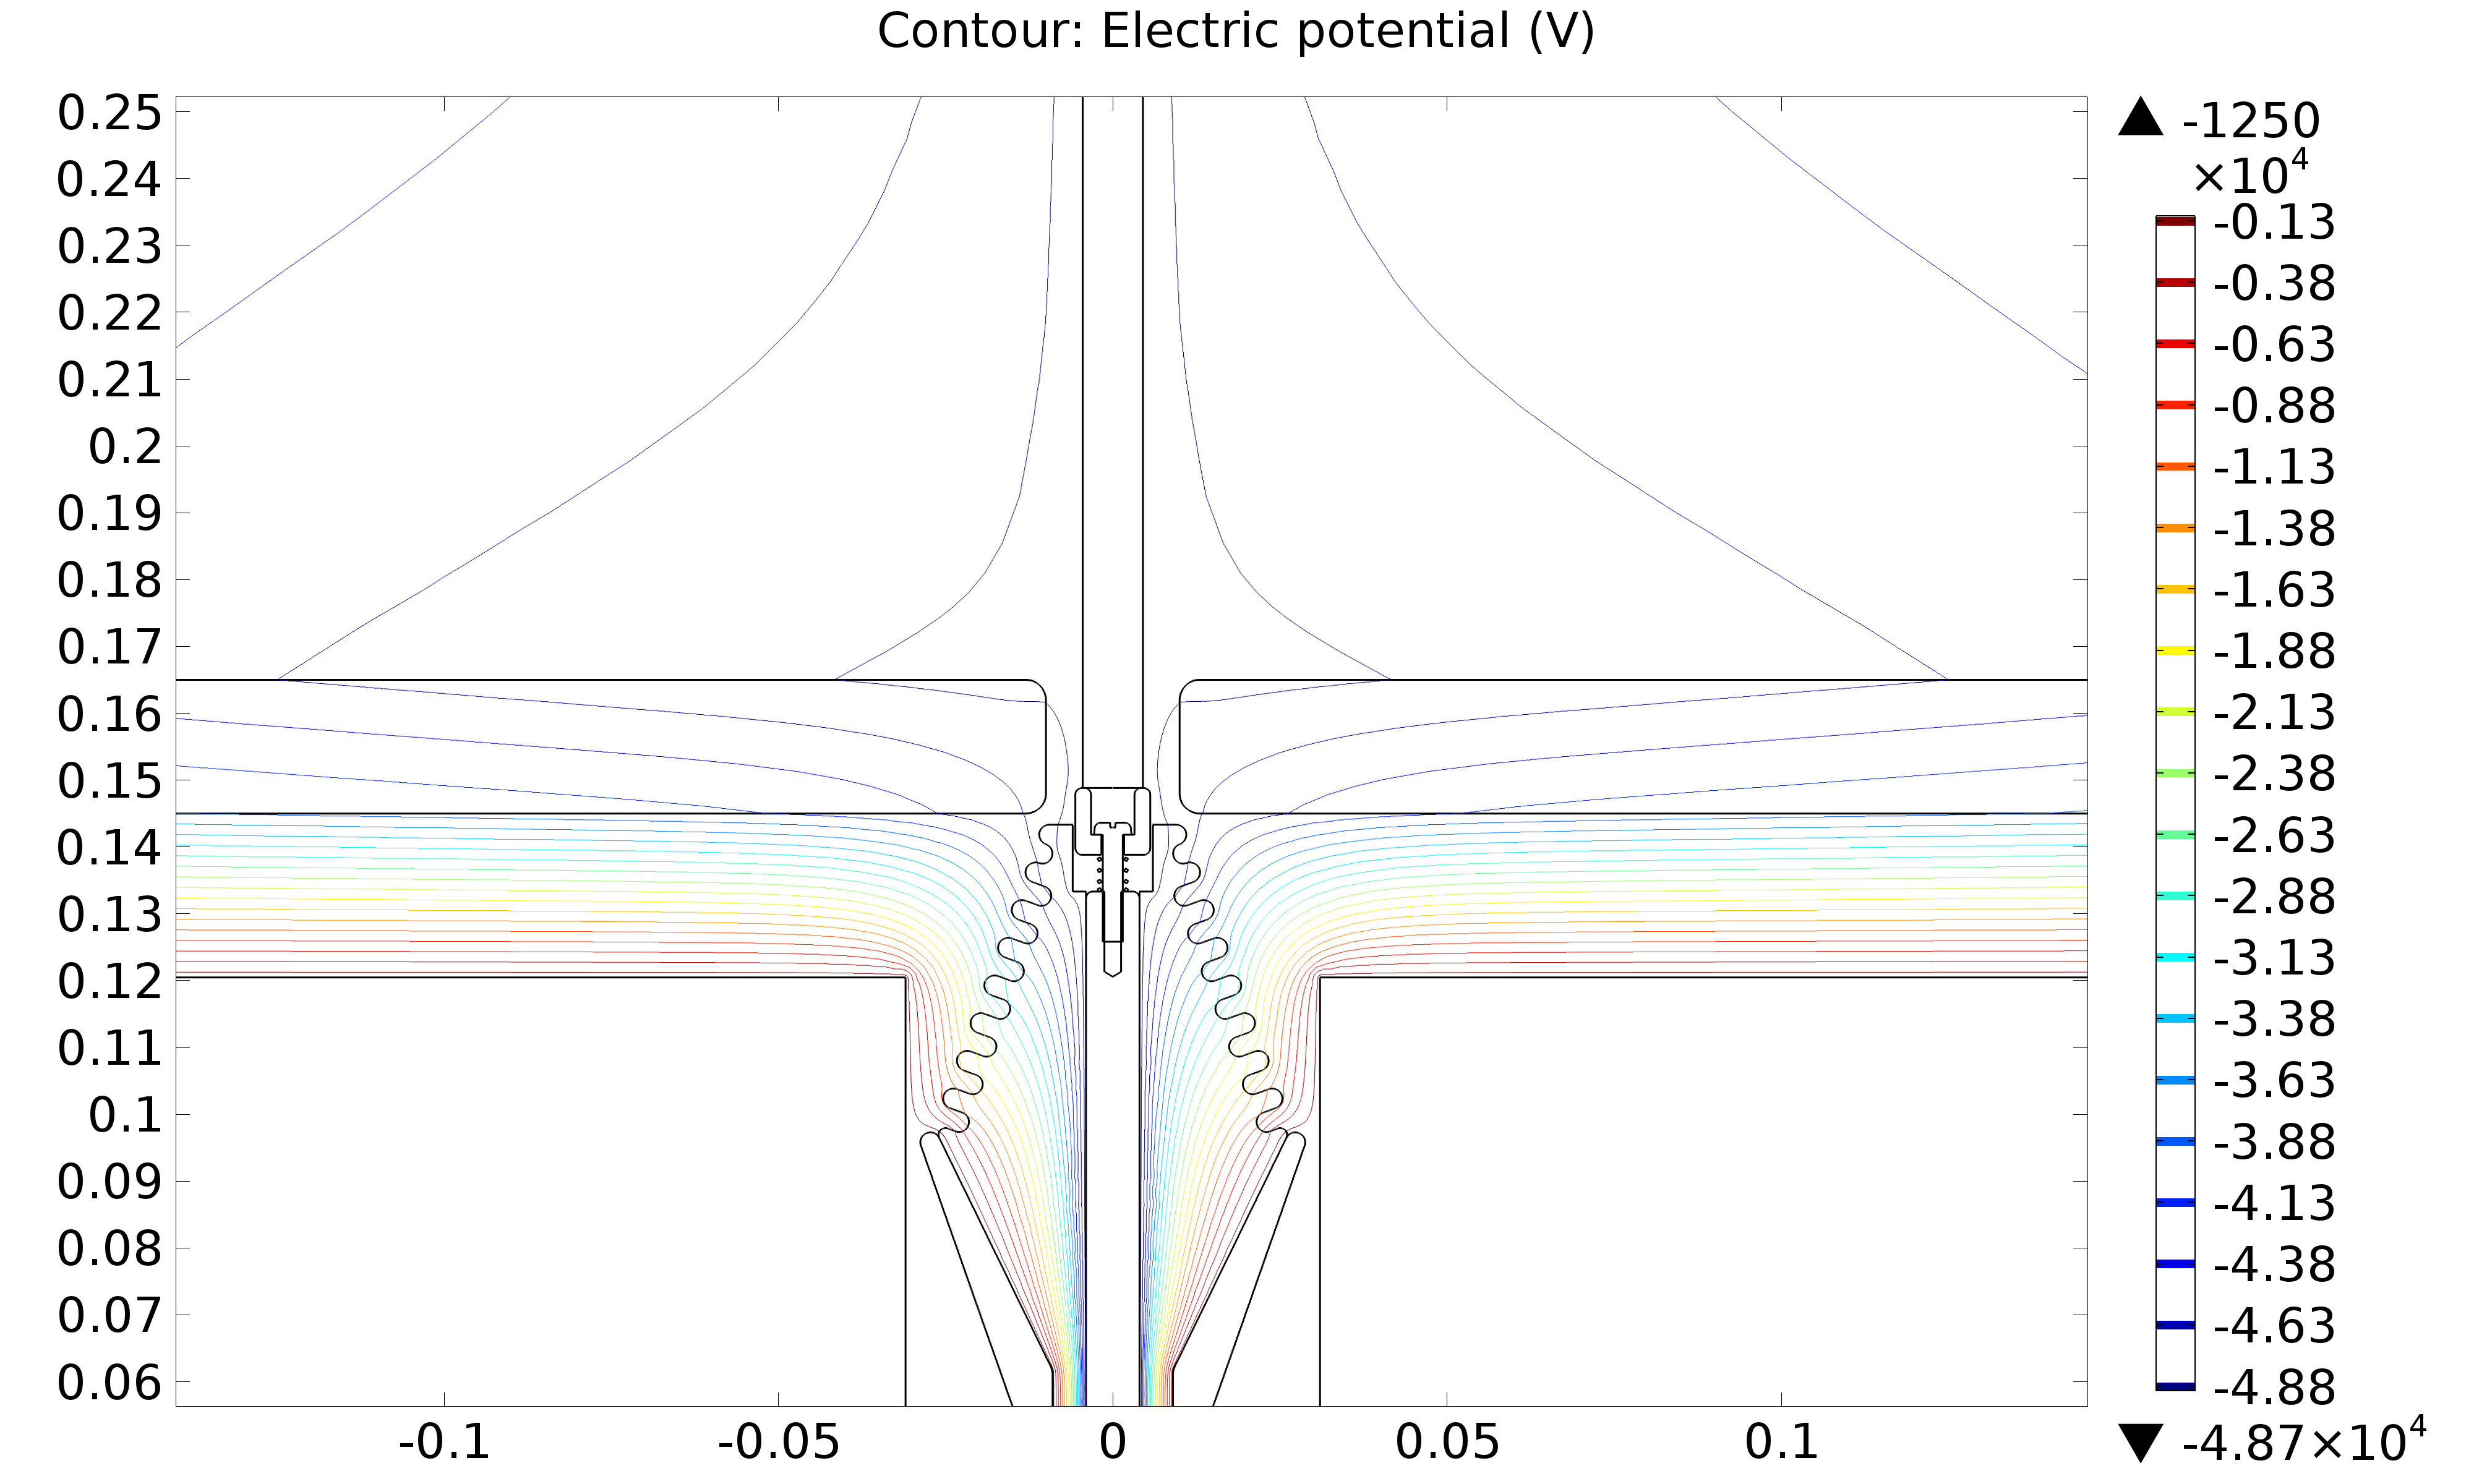
\includegraphics[width=0.45\textwidth]{img/HVFT_with_drift.png}
\caption{Design (left) and Comsol simulation (right) of the HVFT to be used in NEXT-DEMO.} \label{fig:hvft1}
\end{figure}

A key part on that design was the cryo-fitting components to create gas tight seals as all different parts of the HVFT are sealed using this technique.

%\begin{figure}[h!]
%\centering
%\includegraphics[width=0.45\textwidth]{img/cryofit1.jpg}
%\includegraphics[width=0.45\textwidth]{img/cryofit2.jpg}
%\caption{Test for the cryofit sealing. Left image shows the position of the HDPE against the outer vessel. Right image shows the inner steel conductor that will seal agains the inner hole of the HDPE.} \label{fig:hvft2}
%\end{figure}

%During assebly the feedthroughs will be separated from the main vessel and that can represent a safety issue. In order to avoid any possible damage to the people involved in the assembly the next protocol must be followed:
%
%\begin{itemize}
%\item The high voltage feedthrough (HHVFT) has to be completely disconnected from the HHV modules when putting them in place.
%\item Once they have been put in its place in the detector they can be connected to the high voltages modules.
%\item Only authorized people should be able to manipulate modules output voltage manually. Normal user should set the voltage using the slow control system as it is defined in the shifter manual.
%\end{itemize}

In the other hand, a few considerations need to be taken into account when operating the detector:

\begin{itemize}
\item The HHV modules need to be grounded using a proper connexion to the rack frame. This connexion should be check periodically to ensure the quality of the connexion.
\item The cable need to be support with a flexible/movable structure at the top  of the lead castle that will allow to hold the cable when opening/closing the castle without damaging the cable.
\end{itemize}

\subsection{Cathode grid}

The cathode grid consist of a stainless steel frame with wires to fix the potential. Figure \ref{fig:cath} show a detail of the cathode frame with the grooves for fixing the wires and the bronze tensioners.

\begin{figure}[h!]
\centering
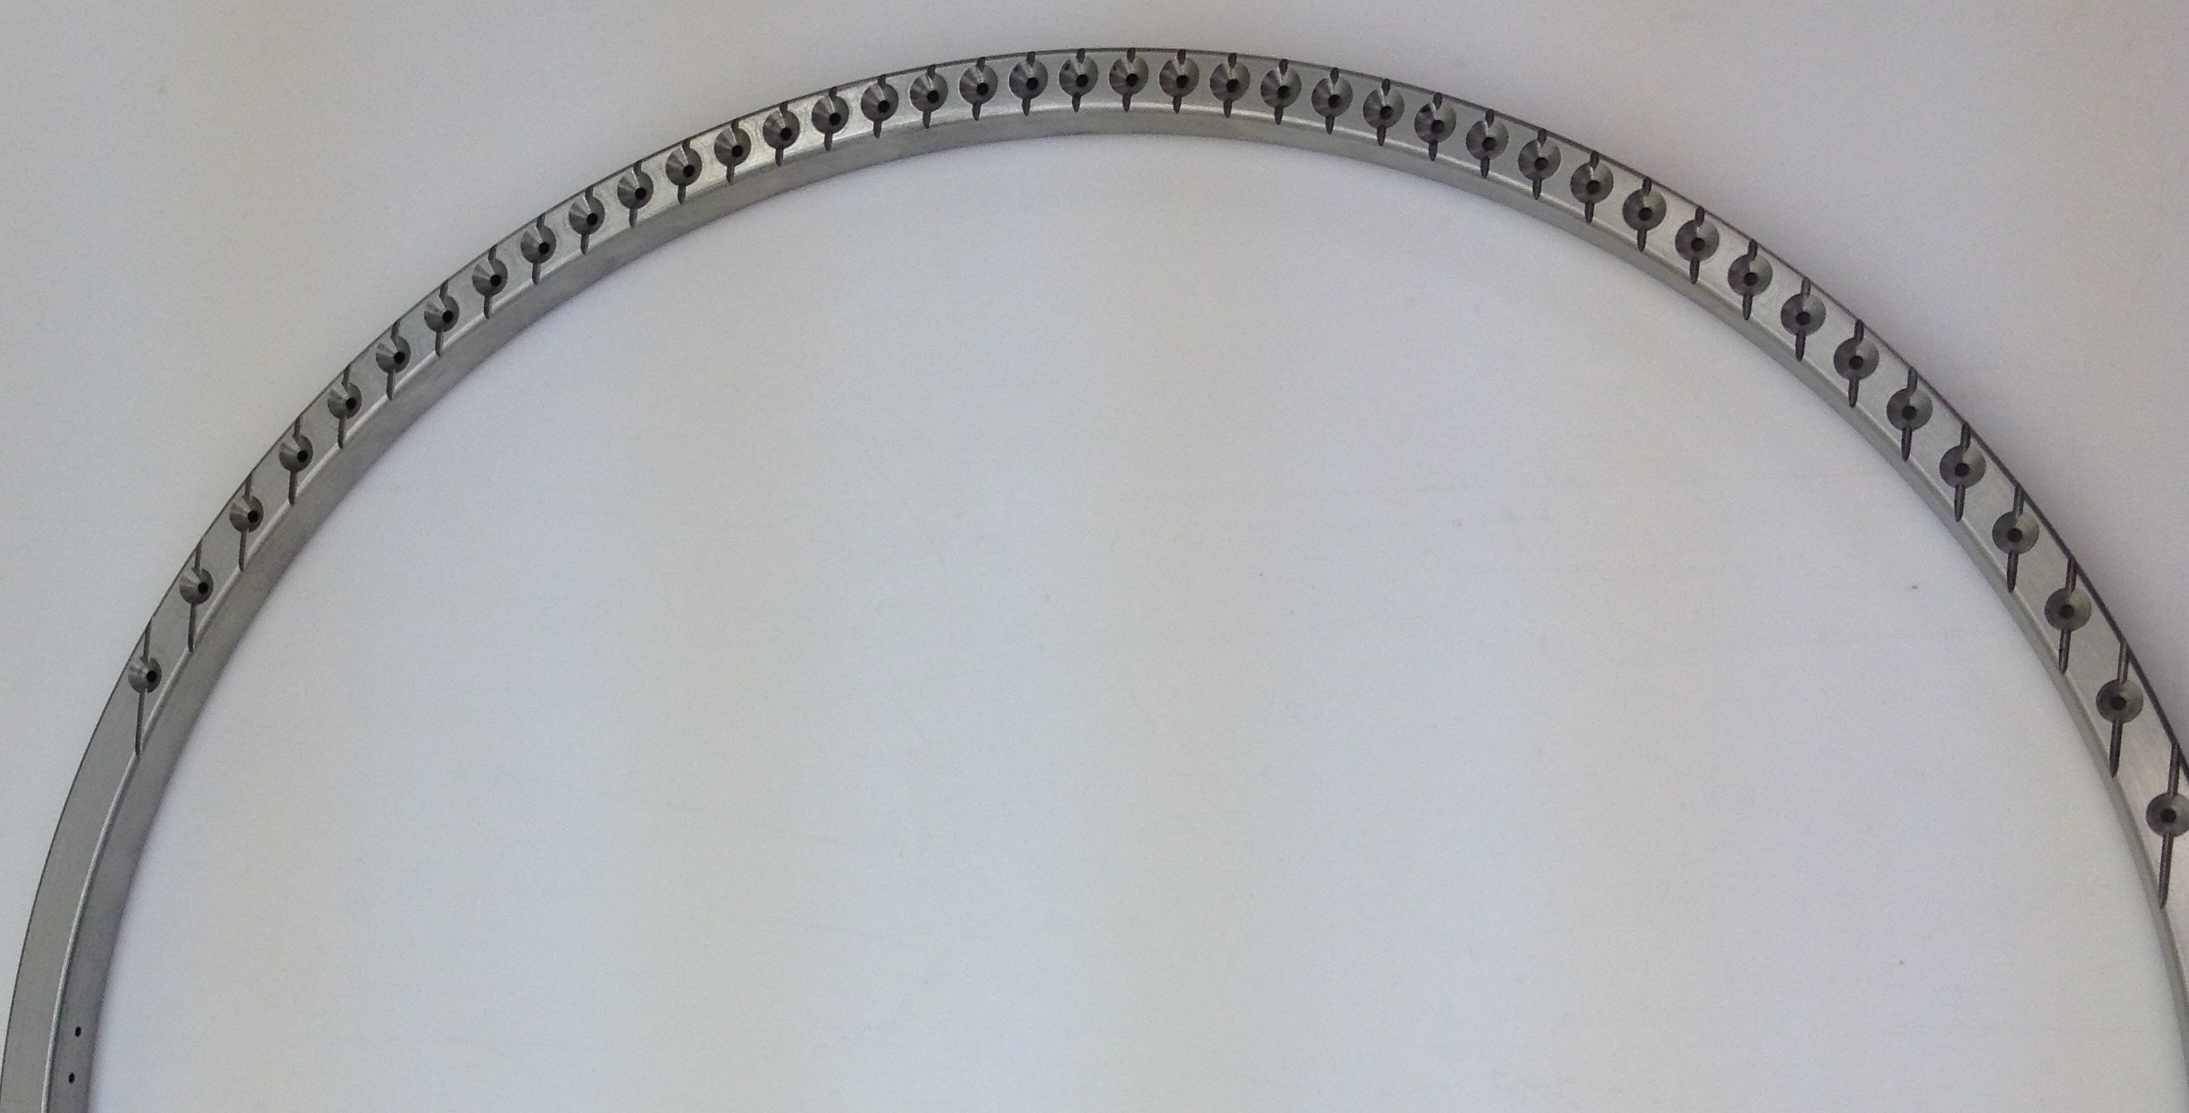
\includegraphics[width=0.45\textwidth]{img/cathode_1.jpg}
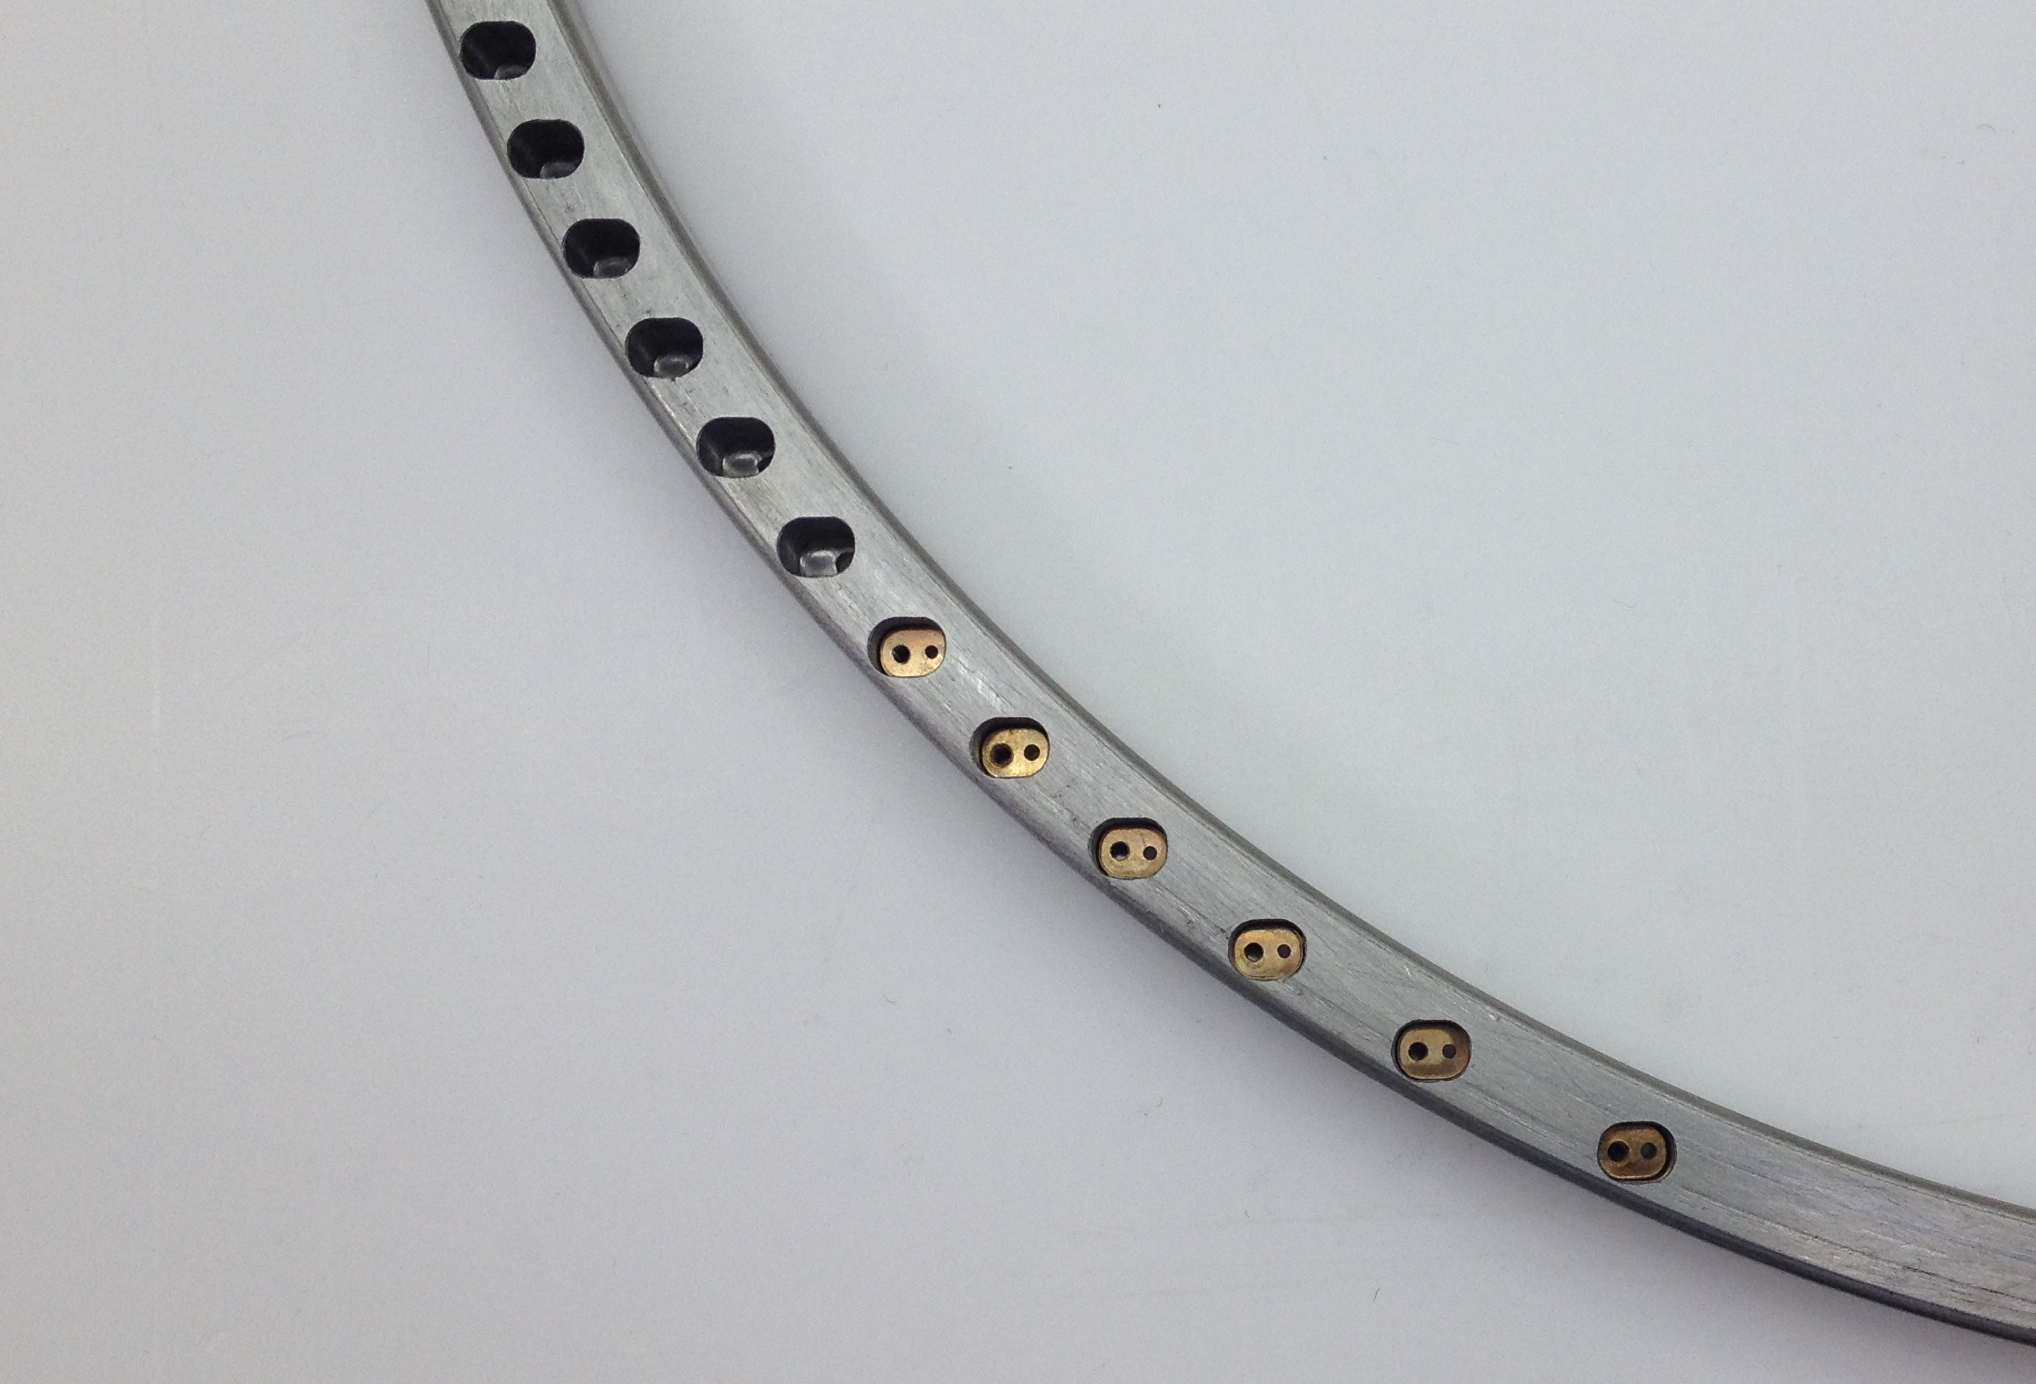
\includegraphics[width=0.45\textwidth]{img/cathode_tensioners.jpg}
\caption{Cathode frame (left) with a detail of the groves for fixing the wires. The bronze tensioners (left) will be used to strength avery wire at the right tension.} \label{fig:cath}
\end{figure}


%No safety issues have been identified with this component of the field cage.


\subsection{Electroluminescent region}

The electroluminescent region is the amplification region of the detector and it is designed to work with the highest electric field.
It consist of a steel mesh grid and a fused silica plate both supported by a HDPE frame.

The main parts of the Electroluminescent region are the mesh and the anode plate. The anode consists in a plate of fused silica coated with ITO in one side and TPB in the other. 

Figure \ref{fig:el} shows details of the different parts of the electroluminescent region.

\begin{figure}[h!]
\centering
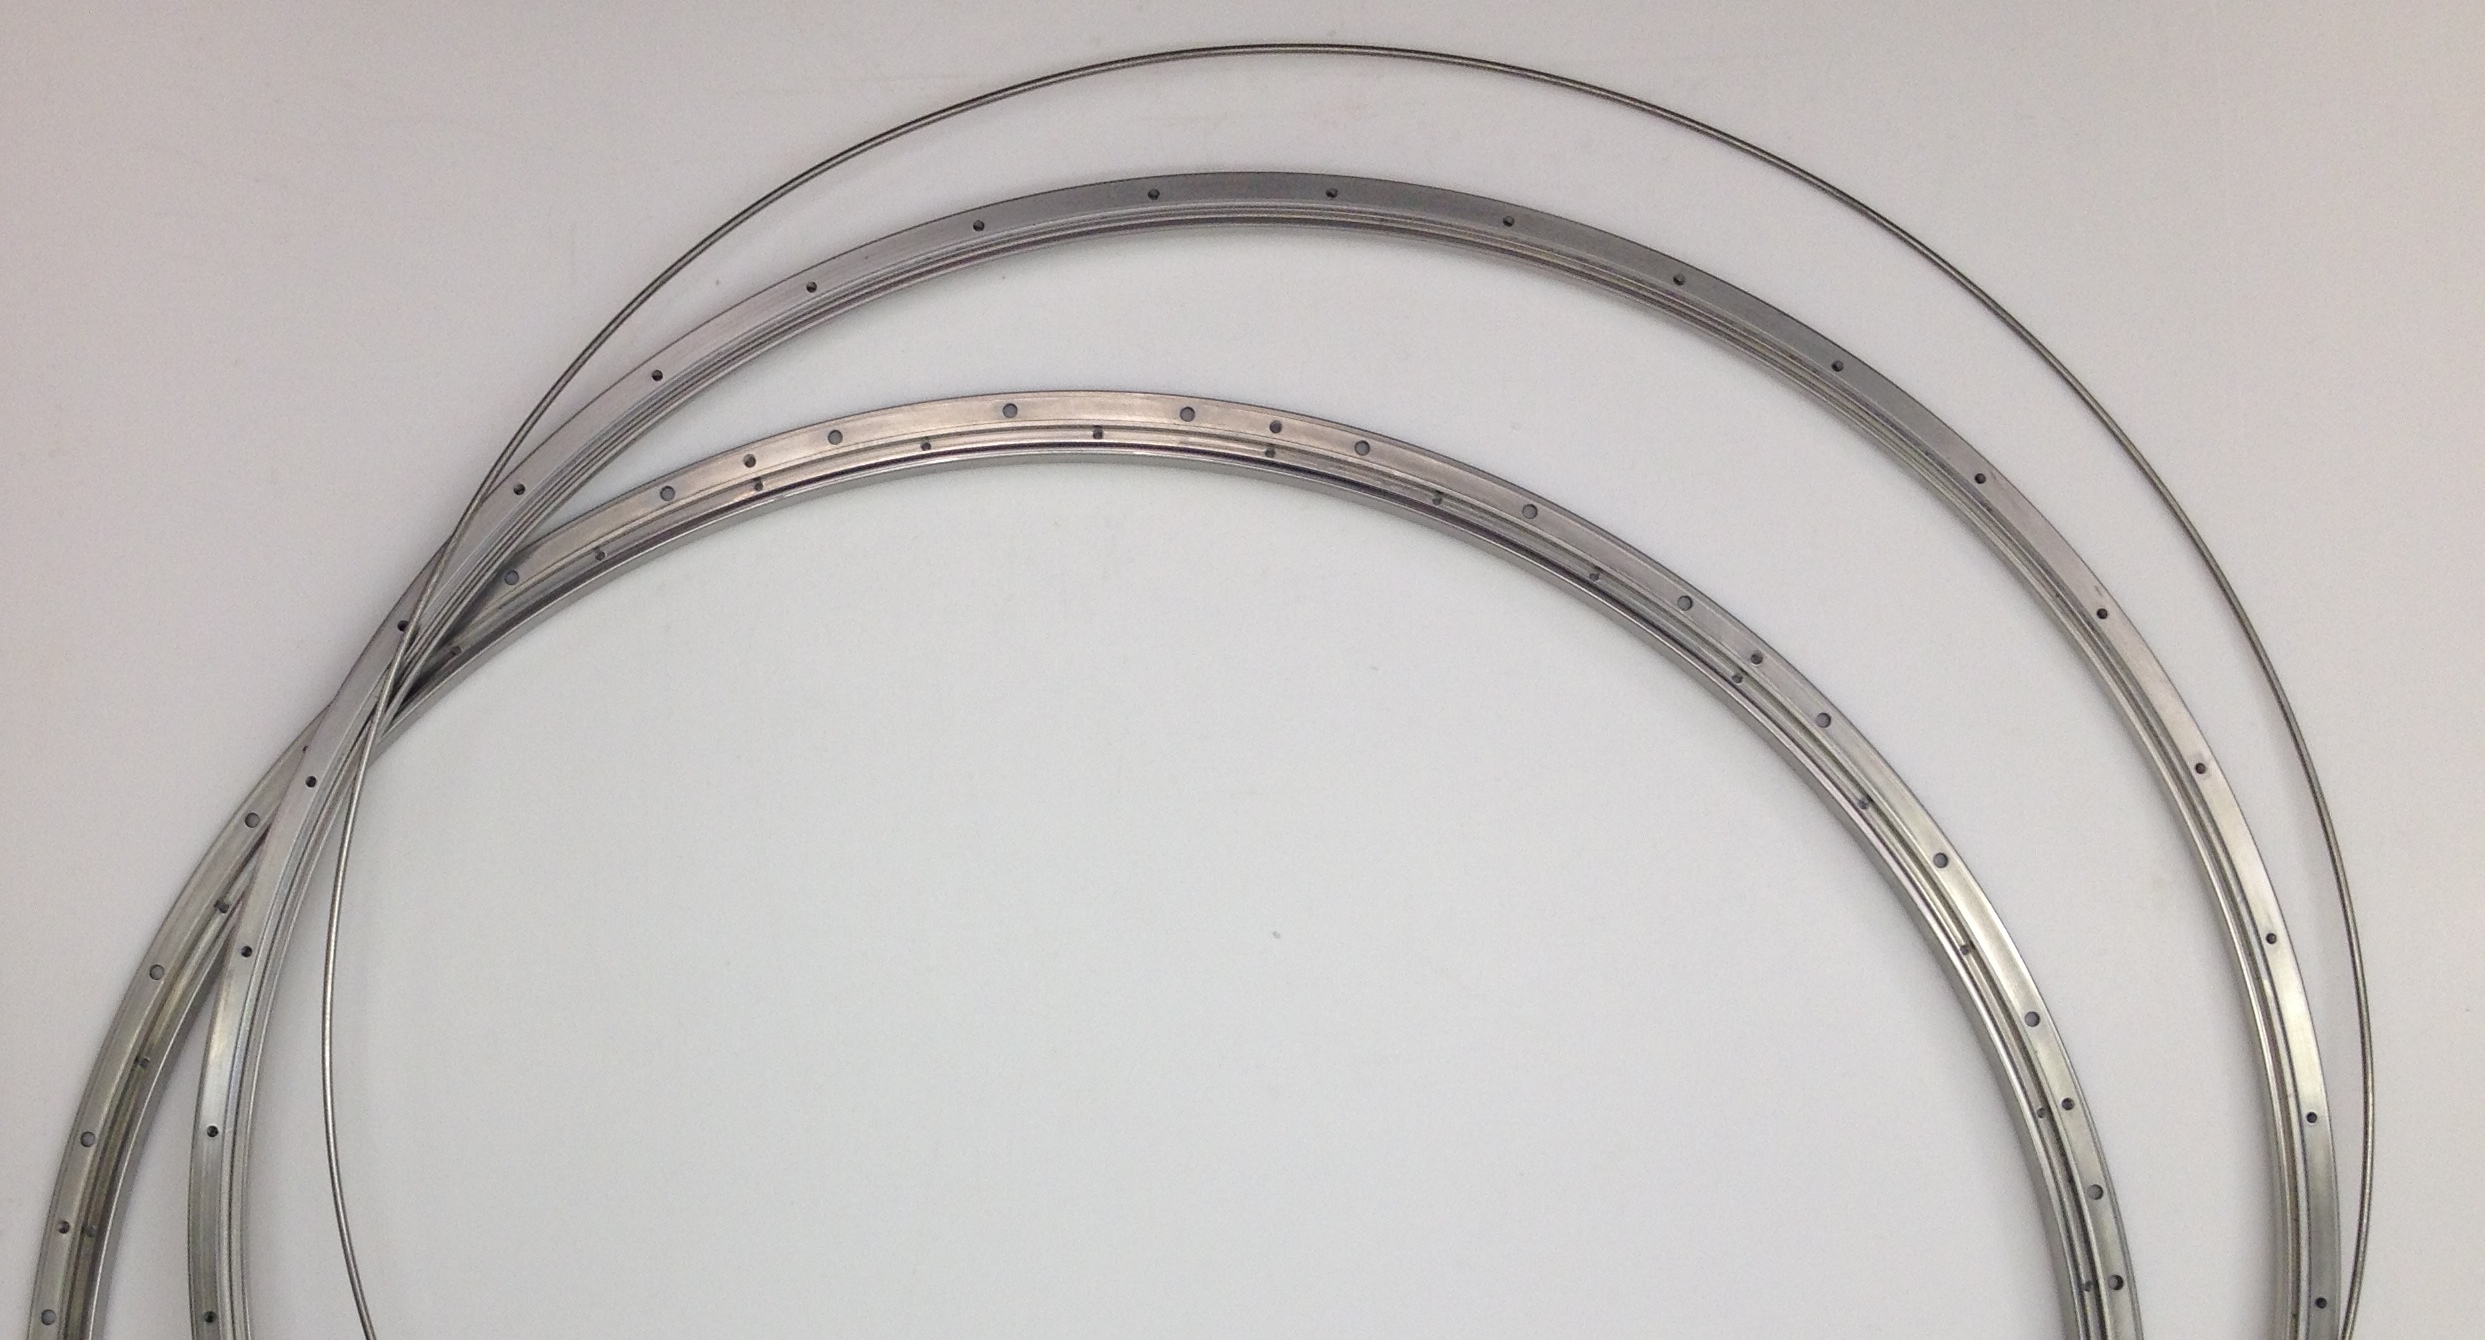
\includegraphics[width=0.45\textwidth]{img/mesh_grid_1.jpg}
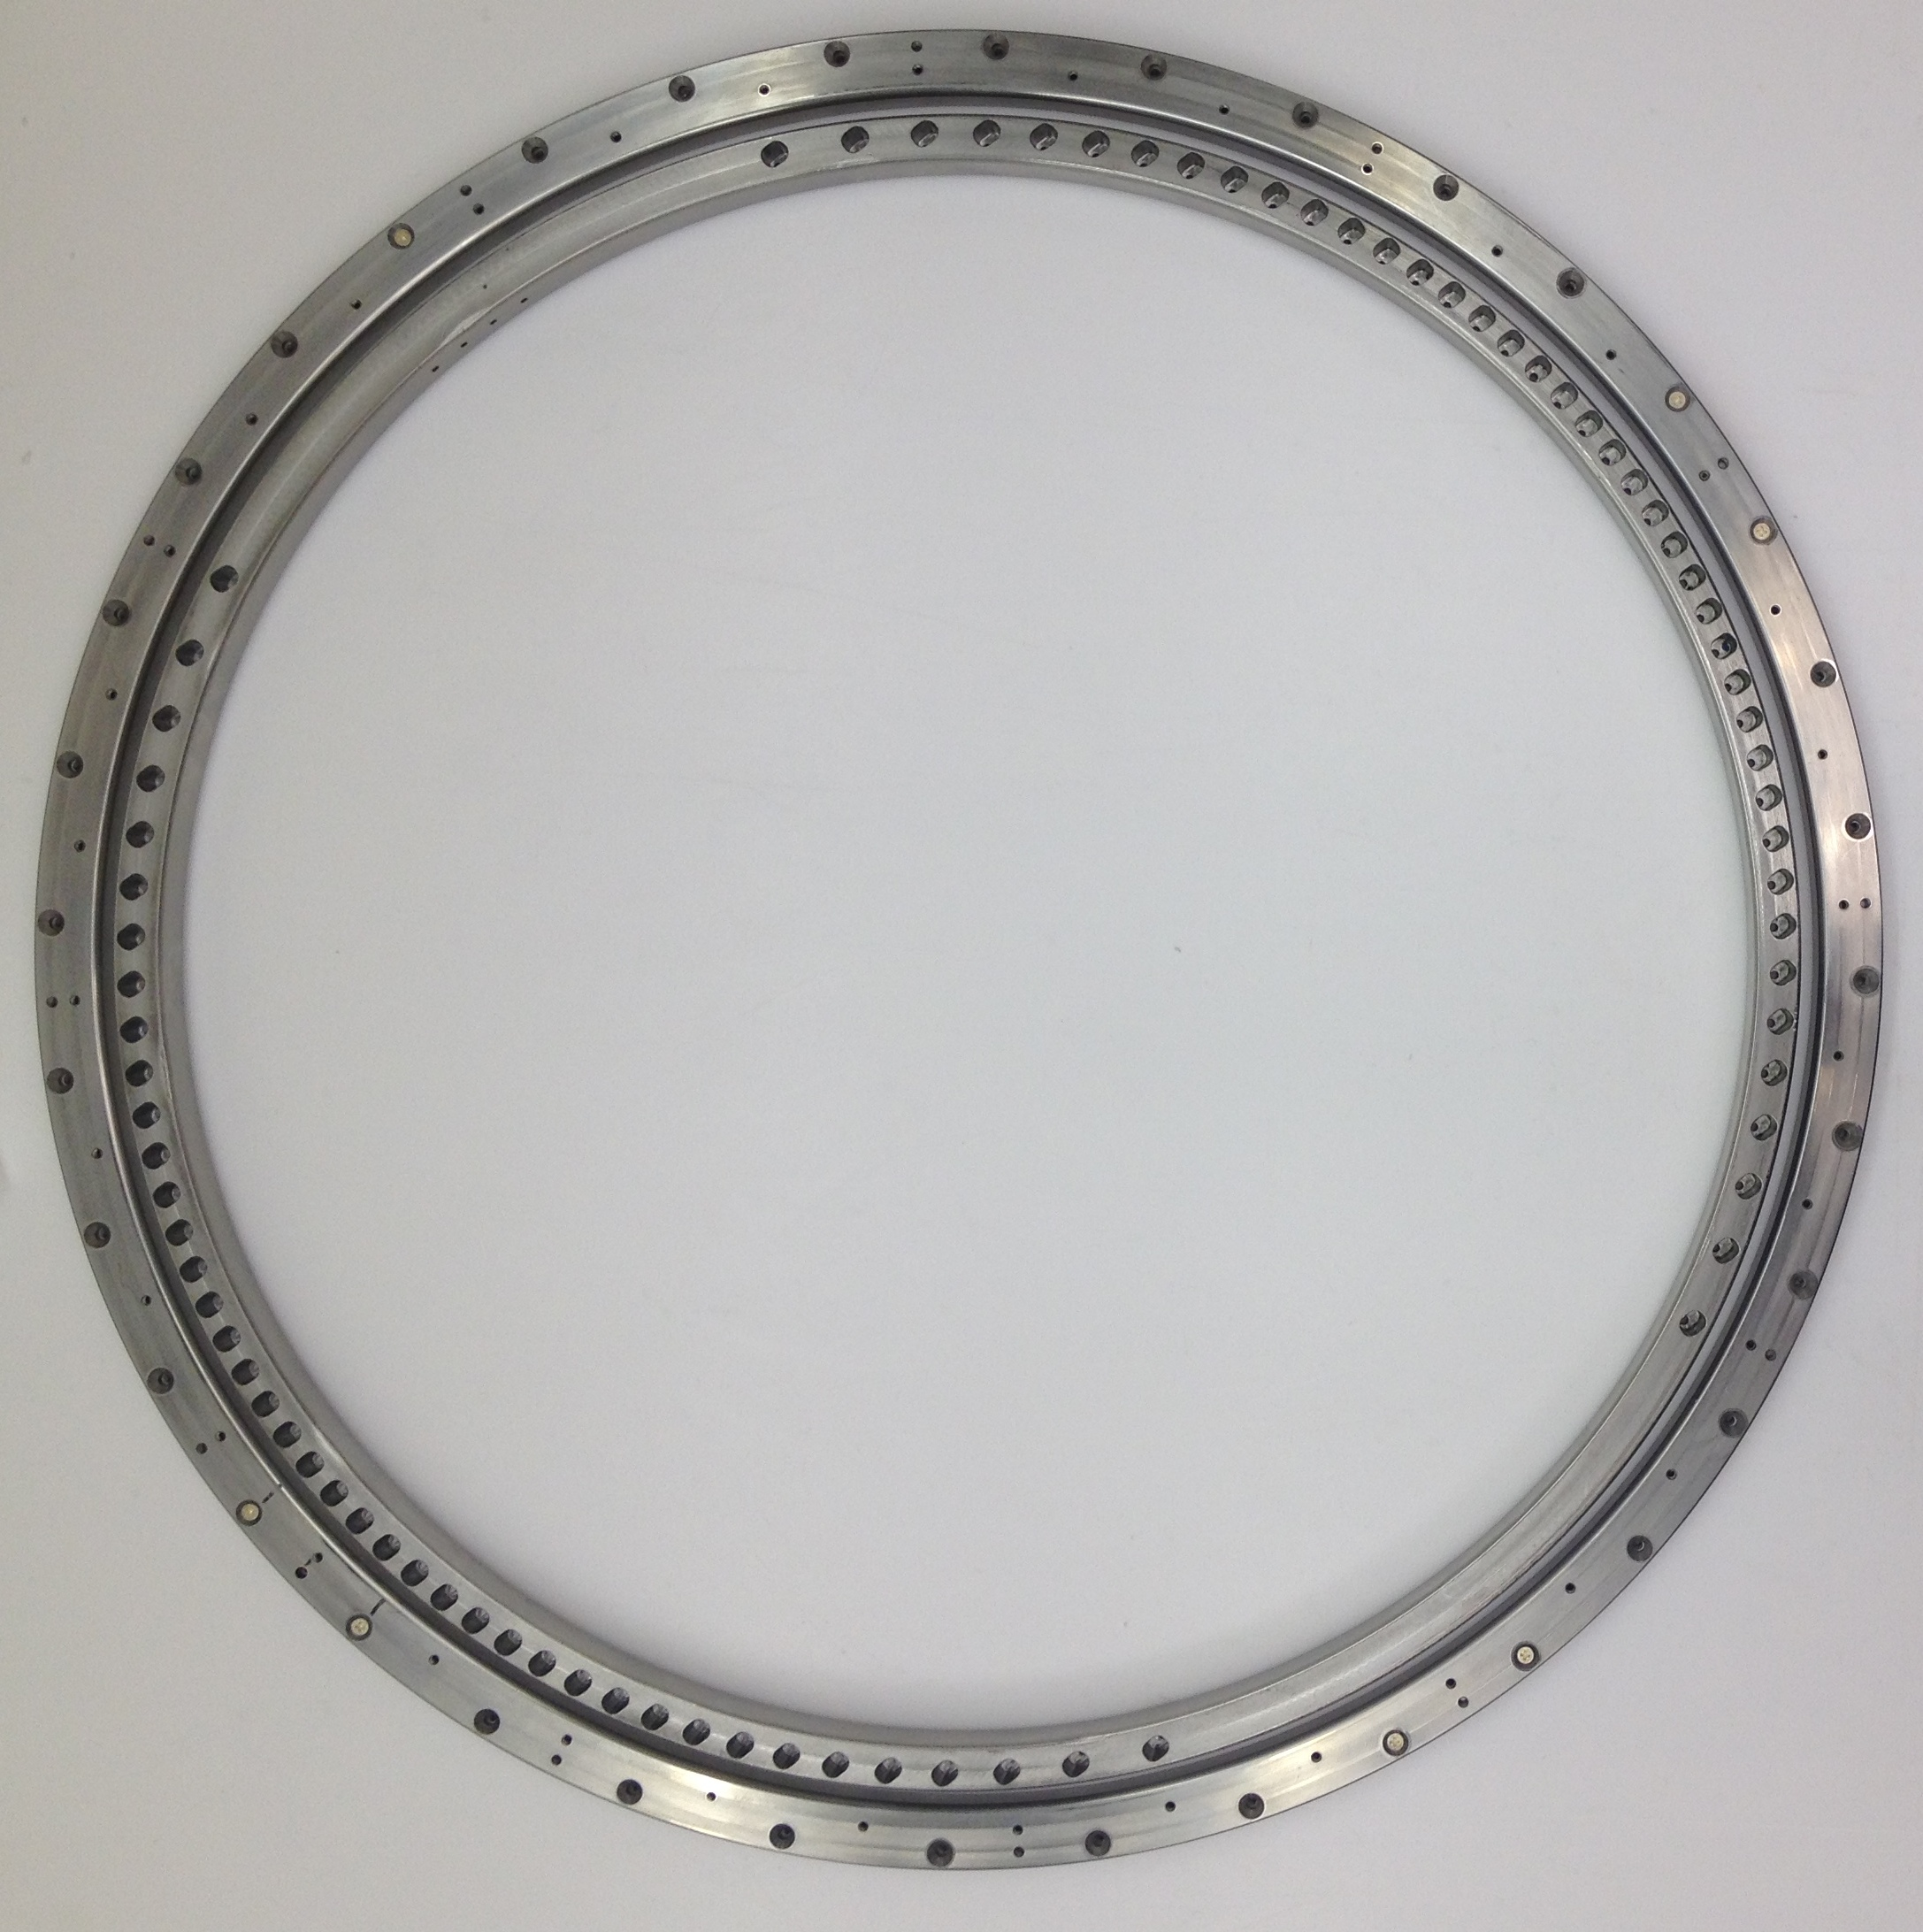
\includegraphics[width=0.45\textwidth]{img/SS_grids_1.jpg}
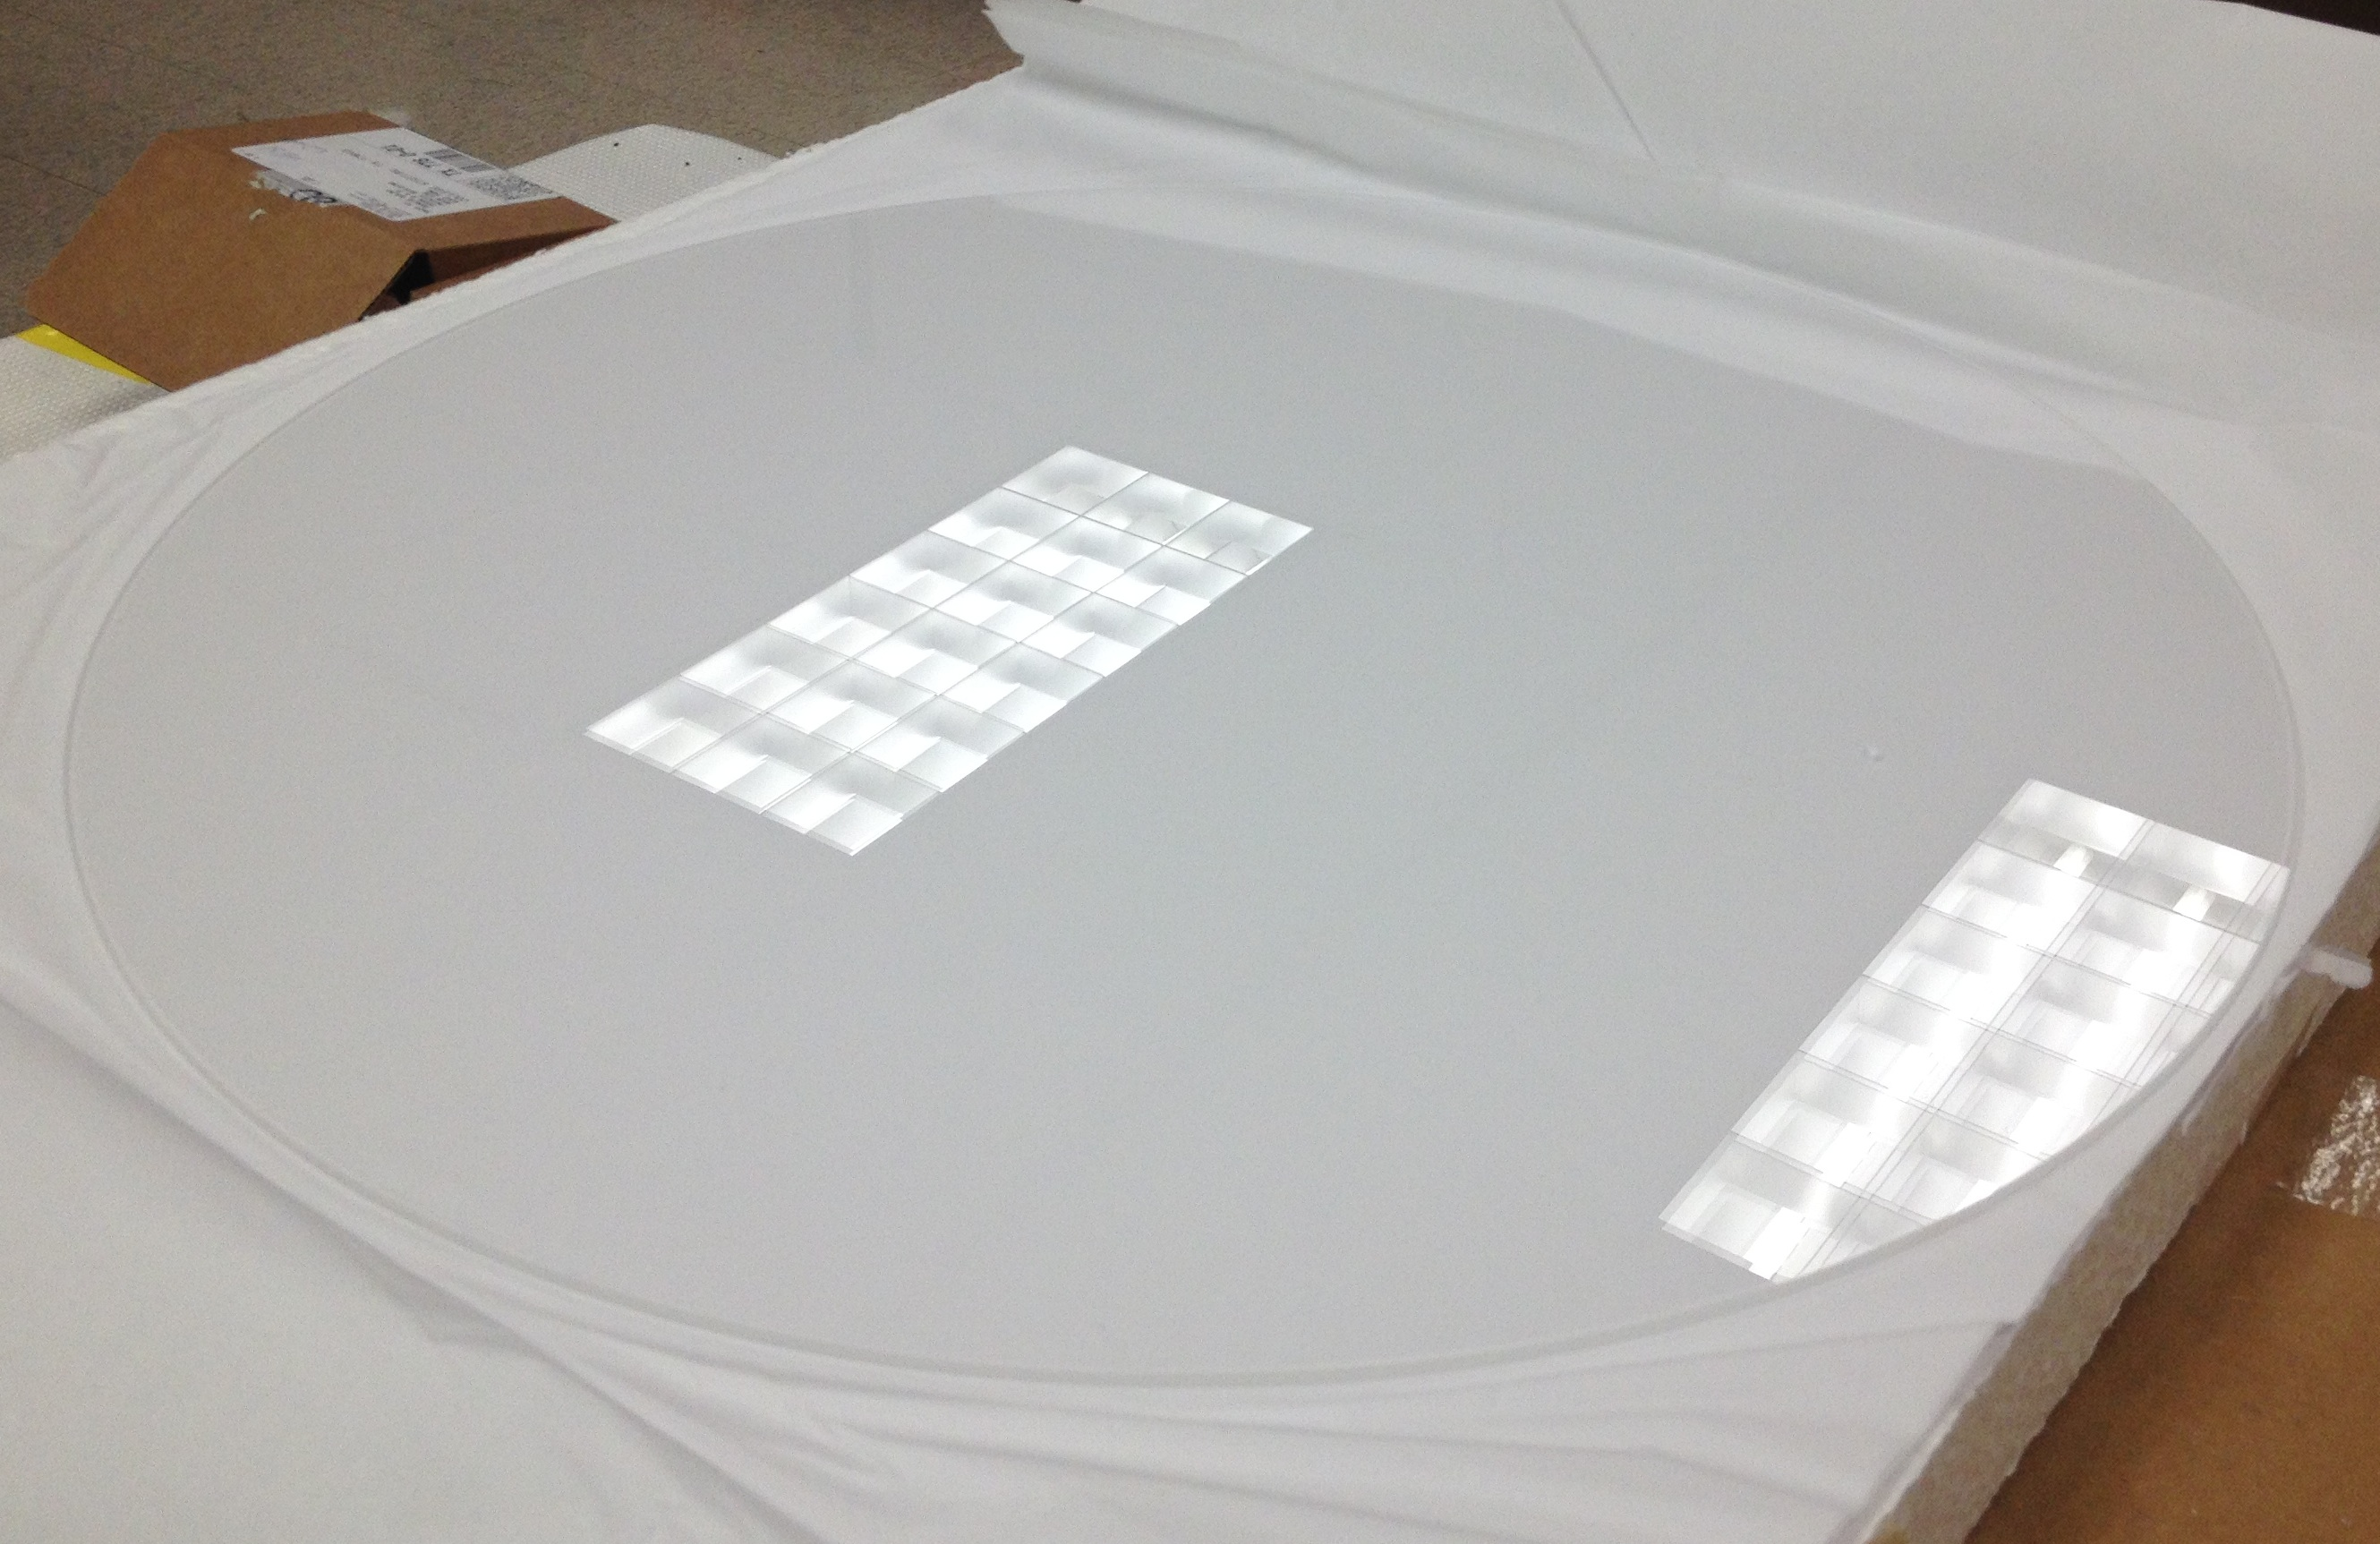
\includegraphics[width=0.45\textwidth]{img/SiO2_uncoated.jpg}
\caption{Top pictures show the diferent frames used for assembly and tension the gate mesh. Bottom is a picture of the fused silica plate before coating with ITO} \label{fig:el}
\end{figure}





%Due to the intensity of the electric field sparks may occur while operating the detector but they will happen inside the detector and so they do not represent a safety issue.

%When installing the detector the fused silica plate needs to be treated very carefull. Only people authorized by the experiment may be allow to do that.


%\section{Installation, schedule, and possible bottle necks}
%
%The time planning for  the NEW field cage ready is illustrated in Fig. \ref{fig:gantt}. It shows that the field cage could be ready by the end of July. 
%In the other hand, there exist a possible bottleneck related with the test in NEXT-DEMO. If that test fails the design of the buffer, HVFT or both will need to be redesigned and tested again. That will imply a general delay of at least one to two months in the delivery.
%
%\begin{figure}[h!]
%\centering
%\includegraphics[width=0.99\textwidth]{img/ganttchart.pdf}
%\caption{Planning to have the NEW field cage ready.} \label{fig:gantt}
%\end{figure}
%
%

